\documentclass[10pt,aspectratio=43]{beamer}

% ── packages ────────────────────────────────────────────────────────────────
\usepackage{graphicx}
\usepackage{booktabs}
\usepackage{multirow}
\usepackage{adjustbox}
\usepackage{amsmath,amssymb}
\usepackage{tikz}
\usepackage{xcolor}
\usepackage{array}
\usepackage{tabularx}
\usepackage{lmodern}
\usepackage{microtype}
\usetikzlibrary{positioning,shapes.geometric,arrows.meta,calc,fit,backgrounds}

% ── Elegant Slides colour palette ───────────────────────────────────────────
\definecolor{primary}{HTML}{08457E}      % deep navy
\definecolor{secondary}{HTML}{B8860B}    % dark gold
\definecolor{tertiary}{HTML}{B22222}     % firebrick (alert)
\definecolor{lightprimary}{HTML}{D6E4F0} % pale navy fill
\definecolor{lightgold}{HTML}{FFF8DC}    % pale gold fill
\definecolor{lightred}{HTML}{FAEAEA}     % pale red fill
\definecolor{lightgreen}{HTML}{E8F5E9}   % pale green fill
\definecolor{successgreen}{HTML}{2E7D32}
\definecolor{pipelineamber}{HTML}{B8860B}
\definecolor{pipelinegreen}{HTML}{1B5E20}
\definecolor{pipelinered}{HTML}{B71C1C}
\definecolor{steelblue}{HTML}{4A90C4}
\definecolor{blockbg}{HTML}{EBF3FB}

% ── Elegant Slides theme (replicated) ───────────────────────────────────────
\usetheme{default}
\useinnertheme{default}
\useoutertheme{default}
\usefonttheme{professionalfonts}

% frametitle: thin navy bar, left-aligned
\setbeamertemplate{frametitle}{%
  \vspace{-0.10cm}
  {\usebeamerfont{frametitle}\usebeamercolor[fg]{frametitle}\insertframetitle}%
  \ifx\insertframesubtitle\@empty\else
    \\[0pt]{\usebeamerfont{framesubtitle}\usebeamercolor[fg]{framesubtitle}\insertframesubtitle}%
  \fi
  \vspace{0.01cm}
  {\color{secondary}\hrule height 0.6pt}
  \vspace{-0.05cm}
}

% footline: left=author | centre=title | right=page/total + section dots
\setbeamertemplate{footline}{%
  \leavevmode%
  \hbox{%
    \begin{beamercolorbox}[wd=0.28\paperwidth,ht=2.0ex,dp=1ex,leftskip=4pt]{footline left}%
      \usebeamerfont{footline}\textcolor{primary!70}{\insertshortauthor}%
    \end{beamercolorbox}%
    \begin{beamercolorbox}[wd=0.44\paperwidth,ht=2.0ex,dp=1ex,center]{footline centre}%
      \usebeamerfont{footline}\textcolor{primary!60}{\insertshorttitle}%
    \end{beamercolorbox}%
    \begin{beamercolorbox}[wd=0.28\paperwidth,ht=2.0ex,dp=1ex,rightskip=4pt,right]{footline right}%
      \usebeamerfont{footline}\textcolor{primary!70}{\insertframenumber\,/\,\inserttotalframenumber}%
    \end{beamercolorbox}%
  }%
  \vskip0pt%
}

% section page: big section number + title
\setbeamertemplate{section page}{%
  \begin{center}
    \vspace{1.2cm}
    {\color{secondary}\fontsize{36}{40}\selectfont\textbf{\thesection}}\\[0.3cm]
    {\color{primary}\Large\textbf{\insertsection}}\\[0.2cm]
    {\color{secondary}\hrule height 0.8pt}
  \end{center}
}

% ── widen content body: narrow side margins, use full slide width ───────────
\setbeamersize{text margin left=6mm, text margin right=6mm}
% tighten two-column gutter so columns use the widened body
\setlength{\columnsep}{6mm}

\setbeamertemplate{navigation symbols}{}
\setbeamertemplate{itemize item}{\color{secondary}\textbullet}
\setbeamertemplate{itemize subitem}{\color{secondary!70}$\circ$}
\setbeamertemplate{enumerate item}{\color{primary}\textbf{\insertenumlabel.}}

% colours
\setbeamercolor{frametitle}{fg=primary}
\setbeamercolor{framesubtitle}{fg=secondary}
\setbeamercolor{normal text}{fg=black!88}
\setbeamercolor{background canvas}{bg=white}
\setbeamercolor{block title}{fg=white, bg=primary}
\setbeamercolor{block body}{fg=black, bg=blockbg}
\setbeamercolor{block title alerted}{fg=white, bg=tertiary}
\setbeamercolor{block body alerted}{fg=black, bg=lightred}
\setbeamercolor{block title example}{fg=white, bg=successgreen}
\setbeamercolor{block body example}{fg=black, bg=lightgreen}
\setbeamercolor{alerted text}{fg=tertiary}
\setbeamercolor{itemize item}{fg=secondary}
\setbeamercolor{enumerate item}{fg=primary}

% fonts
\setbeamerfont{title}{size=\Large, series=\bfseries}
\setbeamerfont{subtitle}{size=\normalsize, series=\normalfont}
\setbeamerfont{frametitle}{size=\large, series=\bfseries}
\setbeamerfont{framesubtitle}{size=\small, series=\normalfont}
\setbeamerfont{block title}{size=\small, series=\bfseries}
\setbeamerfont{footline}{size=\tiny}
\setbeamerfont{itemize/enumerate body}{size=\small}
\setbeamerfont{itemize/enumerate subbody}{size=\footnotesize}

% title page
\setbeamertemplate{title page}{%
  \vspace{0.6cm}
  \begin{center}
    {\color{primary}\Large\textbf{\inserttitle}}\\[0.25cm]
    {\color{secondary}\normalsize\insertsubtitle}\\[0.5cm]
    {\color{primary!60}\hrule height 0.6pt}\\[0.4cm]
    {\small\insertauthor}\\[0.1cm]
    {\footnotesize\color{primary!70}\insertinstitute}\\[0.3cm]
    
\includegraphics[height=1.6cm]{pdeulogo.png}\\[0.2cm]
    {\footnotesize\color{primary!60}\insertdate}
  \end{center}
}

% ── metadata ────────────────────────────────────────────────────────────────
\title[NSE Positional Trading System]{A Positional Trading System for NSE India}
\subtitle{Walk-Forward Ensemble Learning, Calibrated Probabilities \& Live API Deployment}
\author[Vishwam K. Shah]{Vishwam K. Shah \quad {\footnotesize(24MAI022)}}
\institute{M.Tech Artificial Intelligence, PDEU \\ {\footnotesize Guided by: Dr.\ Jigarkumar Shah, ICT Department}}
\date{May 2026}

\graphicspath{{images/}{images/plots/}{images/dashboard/}}

% ── helpers ─────────────────────────────────────────────────────────────────
\newcommand{\hl}[1]{\textcolor{primary}{\textbf{#1}}}
\newcommand{\gr}[1]{\textcolor{successgreen}{\textbf{#1}}}
\newcommand{\rd}[1]{\textcolor{tertiary}{\textbf{#1}}}
\newcommand{\gd}[1]{\textcolor{secondary}{\textbf{#1}}}
\newcommand{\vsep}{\vspace{0.04cm}}

% tighten beamer block vertical padding to reduce slide overflow
\addtobeamertemplate{block begin}{}{\vspace{-2pt}}
\addtobeamertemplate{block end}{\vspace{-4pt}}{}
\addtobeamertemplate{block alerted begin}{}{\vspace{-2pt}}
\addtobeamertemplate{block alerted end}{\vspace{-4pt}}{}
\addtobeamertemplate{block example begin}{}{\vspace{-2pt}}
\addtobeamertemplate{block example end}{\vspace{-4pt}}{}
\newcommand{\AS}{\renewcommand{\arraystretch}{1.15}}

% ════════════════════════════════════════════════════════════════════════════
\begin{document}
% ════════════════════════════════════════════════════════════════════════════

% ── SLIDE 1: TITLE ──────────────────────────────────────────────────────────
{
\setbeamertemplate{footline}{}
\begin{frame}[plain]
  \titlepage
\end{frame}
}
\addtocounter{framenumber}{-1}

% ── SLIDE 2: OUTLINE ────────────────────────────────────────────────────────
\begin{frame}{Outline}
  \begin{columns}[t]
    \column{0.50\textwidth}
      \begin{enumerate}\itemsep4pt
        \item[\gd{1.}] Introduction \& Motivation
        \item[\gd{2.}] Problem Statement
        \item[\gd{3.}] Literature Review
        \item[\gd{4.}] Research Objectives
        \item[\gd{5.}] Data \& Feature Engineering
        \item[\gd{6.}] Five-Model Ensemble
        \item[\gd{7.}] Walk-Forward Validation
      \end{enumerate}
    \column{0.50\textwidth}
      \begin{enumerate}\itemsep4pt
        \item[\gd{8.}]  Results: Accuracy, Portfolio, Per-Symbol
        \item[\gd{9.}]  Comparison with Prior Research
        \item[\gd{10.}] Live System \& Dashboard
        \item[\gd{11.}] Case Studies (prior journal work)
        \item[\gd{12.}] Conclusion \& Contributions
        \item[\gd{13.}] Future Work
        \item[\gd{14.}] References
      \end{enumerate}
  \end{columns}
  \vspace{0.25cm}
  {\color{primary!40}\hrule height 0.4pt}
  \vspace{0.10cm}
  {\footnotesize\color{primary!70}
    \textbf{Domain:} Machine Learning $\cdot$ Financial Time Series $\cdot$ Deep Learning Ensemble $\cdot$ Algorithmic Trading $\cdot$ NSE India}
\end{frame}

% ── SLIDE 3: INTRODUCTION ───────────────────────────────────────────────────
\begin{frame}{Introduction}
  \framesubtitle{Motivation \& Literature Gap}
  \begin{columns}[T]
    \column{0.50\textwidth}
      \gd{\textbf{The Deployability Problem}}
      \vsep
      \begin{itemize}\itemsep4pt
        \item NSE prediction is a \emph{deployability} problem, not just a modelling problem
        \item Indian round-trip cost $\approx$ \textbf{40 bps} (STT + exchange + GST + SEBI + slippage)
        \item \textbf{Our result:} gated \textbf{51\%} model (this thesis) beats an ungated \textbf{58\%} baseline after the Indian cost stack \hfill {\scriptsize(see Results, slide 8)}
        \item Real test: does the signal survive brokerage and slippage?
      \end{itemize}
    \column{0.50\textwidth}
      \gd{\textbf{Literature Gap}}
      \vsep
      \begin{itemize}\itemsep4pt
        \item Indian studies report \rd{60--83\%}: mostly single or random splits
        \item Full-panel scalers leak future statistics into training
        \item No prior work uses expanding-window WFV with regime-conditional Sharpe
        \item No prior work gates live capital on paper-trading KPIs
      \end{itemize}
  \end{columns}
\end{frame}

% ── SLIDE 4: PROBLEM STATEMENT ──────────────────────────────────────────────
\begin{frame}{Problem Statement}
  \framesubtitle{What this thesis is trying to solve}
  \begin{columns}[T]
    \column{0.55\textwidth}
      \begin{exampleblock}{Core Problem}
        \small
        Indian-market ML stock-prediction studies report 60--83\% accuracy, yet none demonstrate that their signal survives the \textbf{Indian cost stack} (STT, GST, exchange, SEBI, slippage $\approx$ 40 bps round-trip) under \textbf{leakage-audited walk-forward validation} on a \textbf{realistic universe}.
      \end{exampleblock}
      \vsep
      \gd{\textbf{Three Sub-Problems}}
      \begin{enumerate}\itemsep3pt\small
        \item \textbf{Honest accuracy:} measure direction accuracy under expanding-window WFV without future-statistic leakage
        \item \textbf{Deployable profit:} produce a cost-net Sharpe $>$ 1 across bull/bear/sideways regimes
        \item \textbf{Capital-safe deployment:} gate live capital on objective KPIs, not on point estimates
      \end{enumerate}
    \column{0.45\textwidth}
      \begin{block}{Research Question}
        \small
        \textit{Can a calibrated, gated ensemble of heterogeneous models produce a statistically significant, cost-net positive return on a 100-stock NSE universe under leakage-audited walk-forward validation?}
      \end{block}
      \vsep
      \begin{alertblock}{Scope}
        \footnotesize
        \begin{itemize}\itemsep2pt
          \item NSE 100 stocks (13 sectors)
          \item Daily-bar positional trading
          \item Direction classification (up / down)
          \item No HFT, no F\&O (left to future work)
        \end{itemize}
      \end{alertblock}
  \end{columns}
\end{frame}

% ── SLIDE 5: LEAKAGE ────────────────────────────────────────────────────────
\begin{frame}{Why Reported Accuracies Are Inflated}
  \framesubtitle{The Validation Protocol Problem}
  \begin{columns}[T]
    \column{0.50\textwidth}
      \begin{alertblock}{Controlled Experiment: The Leakage Trap}
        \footnotesize
        \emph{Same code, same data, same model}: only the validation protocol changes:\\[2pt]
        \textbf{Single 60/20/20 split:} \rd{68.28\%}\\
        \textbf{Six-fold expanding WFV:} \hl{50.97\%}\\[2pt]
        The 17-point drop is \textbf{pure protocol}. The high number was \emph{leakage}, not skill.
      \end{alertblock}
      \gd{\textbf{Common Leakage Sources}}
      \begin{itemize}\itemsep1pt\footnotesize
        \item Random splits mix future rows into training
        \item Full-panel scaler leaks test-set statistics
        \item Rolling features computed across split boundary
        \item Single test window cherry-picks one regime
      \end{itemize}
    \column{0.50\textwidth}
      \begin{exampleblock}{Six Audited Controls in This Work}
        \footnotesize
        \begin{itemize}\itemsep1pt
          \item Target: \texttt{shift(-1)} \emph{after} all features
          \item Scaler + PCA refit per fold on train slice only
          \item Global cues shifted +1 day; backward \texttt{merge\_asof}
          \item Feature selection restricted to training slice
          \item Six chronological folds spanning multiple regimes
          \item Fixed random seed 42 per canonical run
        \end{itemize}
      \end{exampleblock}
  \end{columns}
\end{frame}

% ── SLIDE 5: LITERATURE FOUNDATIONAL ────────────────────────────────────────
\begin{frame}{Literature Review}
  \framesubtitle{Foundational Works}
  \begin{columns}[T]
    \column{0.48\textwidth}
      \gd{\textbf{Theoretical Basis}}
      \vsep
      \begin{itemize}\itemsep4pt
        \item \textbf{EMH} (Fama, 1970): calendar and momentum effects are documented violations of semi-strong EMH
        \item \textbf{Walk-Forward WFV} (L\'opez de Prado, 2018): expanding window is the gold standard; catalogues leakage failure modes
        \item \textbf{Stacked Generalisation} (Wolpert, 1992): heterogeneous learners reduce correlated errors
        \item \textbf{Temperature Scaling} (Guo et al., 2017): $\hat{p}=\sigma(z/T^\star)$; fixes over-confidence, preserves argmax
      \end{itemize}
    \column{0.52\textwidth}
      \gd{\textbf{Five Architectures Used}}
      \vsep
      \begin{itemize}\itemsep4pt
        \item \textbf{XGBoost} (Chen \& Guestrin, 2016): regularised tree boosting on tabular features
        \item \textbf{LightGBM} (Ke et al., 2017): leaf-wise growth; efficient on $\sim$200 features
        \item \textbf{BiLSTM} (Hochreiter \& Schmidhuber, 1997): bidirectional; all features are lagged
        \item \textbf{TCN-Transformer} (Bai et al., 2018): dilated causal conv + 4-head attention
        \item \textbf{N-BEATS} (Oreshkin et al., 2020): residual backcast blocks; sigmoid head
      \end{itemize}
  \end{columns}
\end{frame}

% ── SLIDE 6: INDIAN MARKET ──────────────────────────────────────────────────
\begin{frame}{Literature Review}
  \framesubtitle{Indian-Market Prior Work}
  \begin{columns}[T]
    \column{0.58\textwidth}
      \gd{\textbf{Representative Studies}}
      \vsep
      \AS\scriptsize
      \begin{tabular}{p{1.95cm} p{1.25cm} p{0.95cm} p{1.85cm}}
        \toprule
        \textbf{Study} & \textbf{Models} & \textbf{Data} & \textbf{Protocol} \\
        \midrule
        Shah et al.\ (2019)     & ANN, SVM & Survey  & Rand., 56--83\% \\
        Patel et al.\ (2015)    & ANN, SVM & 10 NSE  & Single, 83\% \\
        Long et al.\ (2019)     & CNN-LSTM & CSE     & Single, 58\% \\
        Nabipour et al.\ (2020) & XGB, LSTM & Tehran  & Single, var. \\
        Fischer \& Krauss (2018)& LSTM     & S\&P500 & Walk-fwd, 56\% \\
        \midrule
        \textbf{This work} & \textbf{5-mdl} & \textbf{100 NSE} & \hl{6-fold, 57.25\%} \\
        \bottomrule
      \end{tabular}
    \column{0.42\textwidth}
      \gd{\textbf{Shared Gaps}}
      \vsep
      \begin{itemize}\itemsep3pt
        \item \rd{Small universe}: 5--20 stocks only
        \item \rd{Single / random splits}: no regime coverage
        \item \rd{No brokerage model}: costs ignored
        \item \rd{No calibration}: arbitrary score cuts
        \item \rd{No live layer}: ends at backtest
      \end{itemize}
      \vsep
      \begin{exampleblock}{This Thesis Addresses All Five}
        \scriptsize
        100 symbols $\cdot$ 6-fold WFV $\cdot$ Indian cost stack $\cdot$ temperature scaling $\cdot$ Angel One live layer
      \end{exampleblock}
  \end{columns}
\end{frame}

% ── SLIDE 7: RESEARCH PROBLEM ───────────────────────────────────────────────
\begin{frame}{Research Problem \& Objectives}
  \begin{columns}[T]
    \column{0.50\textwidth}
      \gd{\textbf{Four Research Questions}}
      \vsep
      {\footnotesize Each RQ is \textbf{testable} and answered with evidence in the Results chapter; together they decompose the central question (slide 4) into falsifiable sub-claims.}
      \vsep
      \begin{itemize}\itemsep3pt
        \item \textbf{RQ1:} Trees + DL ensemble $>$ homogeneous models? \hfill {\scriptsize(panel accuracy ablation)}
        \item \textbf{RQ2:} Temperature calibration improves gate reliability? \hfill {\scriptsize(Brier score, bootstrap CI)}
        \item \textbf{RQ3:} Macro cues + NSE calendar add significant signal? \hfill {\scriptsize(feature ablation)}
        \item \textbf{RQ4:} Profitable across bull, sideways, and bear? \hfill {\scriptsize(per-regime Sharpe)}
      \end{itemize}
    \column{0.50\textwidth}
      \gd{\textbf{Four Design Goals}}
      \vsep
      \begin{block}{G1: Leakage-Free Features}
        \footnotesize Every feature strictly prior to NSE open on day $t$.
      \end{block}
      \vspace{0.08cm}
      \begin{block}{G2: Heterogeneous Ensemble + Calibration}
        \footnotesize Five models + logistic meta-learner + temperature scaling.
      \end{block}
      \vspace{0.08cm}
      \begin{block}{G3: Expanding-Window Walk-Forward}
        \footnotesize 6 folds/symbol; train $0.70\to0.95$; 63,082 out-of-sample (OOS) predictions: data the model never saw in training.
      \end{block}
      \vspace{0.08cm}
      \begin{block}{G4: Promotion Gate}
        \footnotesize 7 KPIs must clear before any real capital is deployed.
      \end{block}
  \end{columns}
\end{frame}

% ── SLIDE 8: DATA & UNIVERSE ────────────────────────────────────────────────
\begin{frame}{Data \& Universe}
  \begin{columns}[T]
    \column{0.50\textwidth}
      \gd{\textbf{Universe \& Data Source}}
      \vsep
      \begin{itemize}\itemsep3pt
        \item \hl{100 NSE symbols}: Nifty-50 + Nifty Next-50
        \item 14 sectors: Banking, IT, FMCG, Pharma, Auto, Energy, Metals, Telecom, Cap Goods, Cement, Consumer Durables, Real Estate, Infra, Defence
        \item Date range: \textbf{Jan 2018 -- Apr 2026}
        \item Source: yfinance, incremental parquet cache
      \end{itemize}
      \vsep
      \gd{\textbf{Global Macro Cues (all symbols)}}
      \vsep
      \begin{itemize}\itemsep3pt
        \item S\&P 500, Nasdaq, VIX, DXY, Crude Oil, Nikkei 225
        \item Shifted +1 calendar day; backward \texttt{merge\_asof}
        \item Day-$t$ signal uses only US close from day $t-1$
      \end{itemize}
    \column{0.50\textwidth}
      \gd{\textbf{NSE Calendar Features}}
      \vsep
      \begin{itemize}\itemsep3pt
        \item Days to next F\&O expiry (last Thursday)
        \item Is-expiry-week / is-expiry-day flag
        \item Days to next RBI MPC announcement
        \item Is-RBI-week flag; days to Union Budget
        \item Results-season indicator (quarterly)
      \end{itemize}
      \vsep
      \begin{exampleblock}{Sector Force-Includes}
        \small
        \textbf{IT:} USD/INR returns + Nasdaq daily return\\[2pt]
        \textbf{Banking/NBFC:} Days-to-RBI + DXY + Crude
      \end{exampleblock}
  \end{columns}
\end{frame}

% ── SLIDE 9: FEATURE ENGINEERING ────────────────────────────────────────────
\begin{frame}{Feature Engineering}
  \framesubtitle{$\sim$200 Leakage-Audited Features}
  \begin{columns}[T]
    \column{0.50\textwidth}
      \gd{\textbf{Feature Families}}
      \vsep
      \AS\scriptsize
      \begin{tabular}{lc}
        \toprule
        \textbf{Family} & \textbf{Count} \\
        \midrule
        Price-based (returns, gaps, MA ratios)     & 20 \\
        Technical (MACD, RSI, Bollinger, ADX)      & 50 \\
        Volume (OBV, MFI, VWAP)                    & 15 \\
        Intraday range (candlestick, shadows)       & 15 \\
        Temporal (cyclic day / week / month)        & 15 \\
        Volatility (HV, Parkinson, Garman-Klass)   & 20 \\
        Momentum (multi-period, acceleration)       & 25 \\
        Statistical (skew, kurtosis, ACF)           & 20 \\
        Regime (trend / vol states)                 & 10 \\
        Interaction (non-linear combos)             & 12 \\
        Global cues + NSE calendar                  & 17 \\
        \midrule
        \textbf{Total}                              & $\sim$\textbf{219} \\
        \bottomrule
      \end{tabular}
    \column{0.50\textwidth}
      \gd{\textbf{Leakage Controls}}
      \vsep
      \AS\scriptsize
      \begin{tabular}{p{1.8cm} p{2.8cm}}
        \toprule
        \textbf{Risk} & \textbf{Control} \\
        \midrule
        Target shift      & \texttt{shift(-1)} after features \\
        Scaler fit        & RobustScaler per fold \\
        PCA fit           & PCA per fold, train only \\
        Global cues       & Prior-day backward join \\
        Feature sel.      & Top-50 per fold, train \\
        Temperature $T^\star$ & Fit on val; infer. apply \\
        \bottomrule
      \end{tabular}
      \vsep
      \begin{block}{Model Inputs}
        \footnotesize
        Top-50 PCA components $\to$ tree models.\\
        3D tensor $B \times 20 \times d$ $\to$ deep models.
      \end{block}
  \end{columns}
\end{frame}

% ── SLIDE 10: FIVE-MODEL ENSEMBLE ───────────────────────────────────────────
\begin{frame}{Five-Model Ensemble Committee}
  \begin{columns}[T]
    \column{0.50\textwidth}
      \gd{\textbf{Tree Models: Fast Pass (09:00 IST)}}
      \vsep
      \begin{itemize}\itemsep3pt
        \item \textbf{\textcolor{pipelineamber}{LightGBM}}: 1,000 trees, lr 0.01, depth 5, $\ell_1$/$\ell_2$ reg, early stop 50
        \item \textbf{\textcolor{pipelineamber}{XGBoost}}: 1,000 trees, lr 0.01, depth 5, subsample 0.8
      \end{itemize}
      \vsep
      \gd{\textbf{Deep Models: Overnight (18:00--08:30 IST)}}
      \vsep
      \begin{itemize}\itemsep3pt
        \item \textbf{\textcolor{pipelinegreen}{BiLSTM}}: 2$\times$64 units, seq 20, dropout 0.2
        \item \textbf{\textcolor{pipelinegreen}{TCN-Transformer}}: dilations \{1,2,4\}, kernel 3; 4-head attention
        \item \textbf{\textcolor{pipelinegreen}{N-BEATS}}: residual backcast blocks, sigmoid head
      \end{itemize}
    \column{0.50\textwidth}
      \begin{block}{Logistic Meta-Learner: the Ensemble's Job}
        \small
        Trained on \textbf{out-of-fold} model probabilities. Its purpose is \textbf{automatic per-symbol model selection}: it learns which members to trust and \textbf{down-weights weak ones}. On tabular features the boosters dominate (cf.\ Shwartz-Ziv 2022); the DL members are kept but the meta-learner correctly weights them low: the ensemble \emph{protecting itself} is the contribution, not 5 equal voters.
      \end{block}
      \vsep
      \begin{block}{Temperature Scaling}
        \small
        $\displaystyle T^\star = \arg\min_{T\in[0.05,5]}\,\mathrm{NLL}\!\left(\sigma(z_v/T),\,y_v\right)$\\[3pt]
        $\hat{p} = \sigma\!\left(\mathrm{logit}(p)/T^\star\right)$\\[3pt]
        Preserves argmax: accuracy unchanged.\\[2pt]
        $\sim$2/3 cells: $T^\star\approx 1$; $\sim$1/3: $T^\star<0.9$ (compressed).
      \end{block}
  \end{columns}
\end{frame}

% ── SLIDE 11: WALK-FORWARD VALIDATION ───────────────────────────────────────
\begin{frame}{Walk-Forward Validation Protocol}
  \begin{columns}[T]
    \column{0.50\textwidth}
      \gd{\textbf{Expanding-Window Design}}
      \vsep
      \begin{block}{Fold $k$ split}
        \small
        $r_k = 0.70 + 0.05(k{-}1),\quad k{=}1{\dots}6$\\[2pt]
        $\mathrm{train}_k = \lfloor N\cdot r_k\rfloor$,\; val $=10\%$,\; test $=$ rest
      \end{block}
      \vsep
      \begin{block}{Target (binary, dead-band)}
        \small
        $y_t = \mathbb{1}\!\left[(C_{t+1}-C_t)/C_t \geq \delta\right],\; \delta = 0.004$
      \end{block}
      \vsep
      \begin{exampleblock}{Signal Gate}
        \small
        $\boxed{\,(\hat{p}\geq 0.58)\;\wedge\;(|\widehat{\Delta}|\geq 0.4\%)\,}$\\[3pt]
        Clears $\approx$40 bps round-trip before entry.
      \end{exampleblock}
    \column{0.50\textwidth}
      \gd{\textbf{SBIN: Six Folds}}
      \vsep
      \AS\scriptsize
      \begin{tabular}{ccccc}
        \toprule
        \textbf{Fold} & \textbf{Train} & \textbf{Val} & \textbf{Test} & \textbf{OOS Acc.} \\
        \midrule
        1 (0.70) & 702 & 78  & 112 & 0.500 \\
        2 (0.75) & 753 & 83  & 111 & 0.622 \\
        3 (0.80) & 803 & 89  & 111 & 0.477 \\
        4 (0.85) & 853 & 94  & 112 & 0.661 \\
        5 (0.90) & 903 & 100 & 112 & 0.554 \\
        6 (0.95) & 954 & 105 &  56 & 0.446 \\
        \midrule
        \multicolumn{4}{r}{\textbf{Mean}} & \hl{0.543} \\
        \bottomrule
      \end{tabular}
      \vsep
      \begin{block}{Why Fold Accuracy Varies}
        \footnotesize
        Fold 4 (2024 Q3 bull) = 0.661; Fold 6 (2026 correction) = 0.446. Multi-fold reporting is honest; single-fold cherry-picks a regime.
      \end{block}
  \end{columns}
\end{frame}

% ── SLIDE 12: RESULTS ACCURACY ──────────────────────────────────────────────
\begin{frame}{Results: Out-of-Sample Accuracy}
  \begin{columns}[T]
    \column{0.46\textwidth}
      \gd{\textbf{Panel Summary (100 Symbols)}}
      \vsep
      \AS\scriptsize
      \begin{tabular}{lc}
        \toprule
        \textbf{Metric} & \textbf{Value} \\
        \midrule
        Symbols / folds           & 100 / 6 \\
        Mean accuracy (all days)  & \gr{50.97\%} \\
        Mean F1-score             & \gr{58.79\%} \\
        \midrule
        Bootstrap accuracy (gated) & \gr{57.25\%} \\
        Statistical significance   & \gr{$p<0.05$} \\
        $H_0\!:p=0.5$ rejected    & \gr{Yes} \\
        \bottomrule
      \end{tabular}
      \vsep
      \gd{\textbf{Top-5 by OOS Accuracy}}
      \vsep
      \AS\scriptsize
      \begin{tabular}{llc}
        \toprule
        \textbf{Symbol} & \textbf{Sector} & \textbf{Acc.} \\
        \midrule
        MUTHOOTFIN & Finance & \gr{0.585} \\
        EICHERMOT  & Auto    & \gr{0.580} \\
        EXIDEIND   & Auto    & \gr{0.575} \\
        TORNTPHARM & Pharma  & \gr{0.572} \\
        PERSISTENT & IT      & \gr{0.567} \\
        \bottomrule
      \end{tabular}
    \column{0.54\textwidth}
      \gd{\textbf{Cross-Stock OOS Accuracy: 100 Symbols}}
      \begin{center}
        
\includegraphics[height=5.8cm,keepaspectratio]{cross_stock_comparison.png}
      \end{center}
  \end{columns}
\end{frame}

% ── SLIDE 13: PORTFOLIO BACKTEST ────────────────────────────────────────────
\begin{frame}{Results: Portfolio Backtest}
  \begin{columns}[T]
    \column{0.46\textwidth}
      \gd{\textbf{Top-15, Long-Only, Equal-Weight}}
      \vsep
      \AS\scriptsize
      \begin{tabular}{lc}
        \toprule
        \textbf{Metric} & \textbf{Value} \\
        \midrule
        Period            & Dec 2023 -- Apr 2026 \\
        Total return      & \gr{170.65\%} \\
        Nifty-50          & \rd{$\sim$18\%} \\
        Sharpe ratio      & \gr{1.18} \\
        Max drawdown      & \gr{14.59\%} \\
        \midrule
        \textit{Regime Sharpe:} & \\
        \quad Sideways     & \gr{1.69} \\
        \quad Bear         & \gr{1.67} \\
        \quad Bull         & \gr{1.43} \\
        \midrule
        DM vs Momentum    & \gr{$p < 0.001$} \\
        DM vs AR(1)       & \gr{$p = 0.001$} \\
        DM vs Always-up   & $p=0.92$ (n.s.) \\
        \bottomrule
      \end{tabular}
    \column{0.54\textwidth}
      \gd{\textbf{Direction Accuracy Distribution}}
      \begin{center}
        
\includegraphics[width=0.95\textwidth]{COMBINED_direction_accuracy_distribution.png}
      \end{center}
      {\scriptsize\textit{Mode near 0.52, right tail to 0.59. Panel edge is distributed; no single stock dominates the return.}}
      \vsep
      \begin{block}{Performance Metrics}
        \footnotesize
        $\mathrm{Sharpe} = \dfrac{\mathbb{E}[r_p]-r_f}{\sigma(r_p)}\sqrt{252}$\quad
        $\mathrm{MaxDD} = \min_t \dfrac{V_t-\max_{s\leq t}V_s}{\max_{s\leq t}V_s}$\\[2pt]
        $V_t$: portfolio NAV at $t$.\; DM stat:
        $\mathrm{DM}=\bar d/\sqrt{\widehat{\mathrm{Var}}(\bar d)/n}$,\, $d_t=L_t^{(a)}-L_t^{(b)}$.
      \end{block}
  \end{columns}
\end{frame}

% ── SLIDE 14: COMPARISON ────────────────────────────────────────────────────
\begin{frame}{Comparison with Prior Research}
  \begin{columns}[T]
    \column{0.58\textwidth}
      \gd{\textbf{Head-to-Head}}
      \vsep
      \AS\scriptsize
      \begin{tabular}{p{2.2cm} p{1.0cm} p{2.0cm} p{0.6cm}}
        \toprule
        \textbf{Study} & \textbf{Acc.} & \textbf{Protocol} & \textbf{Live} \\
        \midrule
        Patel et al.\ (2015)     & 83\%     & Single split, 10 NSE  & No \\
        Fischer \& Krauss (2018) & 56\%     & Walk-fwd, S\&P500     & No \\
        Long et al.\ (2019)      & 58\%     & Single split, CNN-LSTM & No \\
        Nabipour et al.\ (2020)  & Var.     & Single split, Tehran  & No \\
        Shah et al.\ (2019)      & 56--83\% & Survey, rand.\ splits  & No \\
        \midrule
        \textbf{This (all)}  & 50.97\%  & \hl{6-fold WFV, 100 NSE} & \hl{Yes} \\
        \textbf{This (gated)}& \gr{57.25\%} & \hl{$p<0.05$ significant} & \hl{Yes} \\
        \bottomrule
      \end{tabular}
      \vsep
      {\scriptsize\textit{51\% all-days vs 83\% single-split is a protocol difference, not a quality gap. Gated accuracy (57.25\%) is statistically significant and cost-aware: no prior Indian study reports either.}}
    \column{0.42\textwidth}
      \gd{\textbf{Key Differentiators}}
      \vsep
      \begin{itemize}\itemsep3pt
        \item Prior studies ignore 40 bps cost; 83\% on paper may be loss-making
        \item Prior: 5--20 stocks; this: 100 large-caps across 14 sectors
        \item No prior Indian study reports Sharpe, max DD, or regime performance
        \item \hl{Fischer \& Krauss (2018)} closest (WFV, S\&P500, 56\%); this achieves 57.25\% gated on NSE, cost-net
      \end{itemize}
  \end{columns}
\end{frame}

% ── SLIDE 15: WHY IT WORKS ──────────────────────────────────────────────────
% ── LIVE PIPELINE ───────────────────────────────────────────────────────────
\begin{frame}{Live System: Deployment Pipeline}
  \begin{columns}[T]
    \column{0.44\textwidth}
      \gd{\textbf{Automated Promotion Gate: 7 KPIs}}
      \vsep
      \AS\scriptsize
      \begin{tabular}{lc}
        \toprule
        \textbf{KPI} & \textbf{Threshold} \\
        \midrule
        Closed trades   & $\geq 40$ \\
        Paper days      & $\geq 20$ \\
        Rolling Sharpe  & $\geq 1.0$ \\
        Max drawdown    & $\leq 10\%$ \\
        Fill rate       & $\geq 90\%$ \\
        Slippage        & $\leq 25$\,bps \\
        Brier drift     & $\leq 0.05$ \\
        \midrule
        \textbf{Logic} & \textbf{ALL must pass} \\
        \bottomrule
      \end{tabular}
      \vsep
      \begin{exampleblock}{Gate Works by Design}
        \footnotesize
        The gate \textbf{fails closed}: until \textbf{every} KPI clears on a clean paper-trading record, real capital stays blocked. The system \textbf{cannot} fail open into live trading.
      \end{exampleblock}
      \vsep
      \begin{block}{Brier Score (calibration KPI)}
        \footnotesize
        $\mathrm{BS}=\tfrac{1}{n}\sum_{t=1}^{n}(\hat p_t-y_t)^2$\quad (lower is better)
      \end{block}
    \column{0.56\textwidth}
      \begin{center}
      \resizebox{\textwidth}{!}{%
      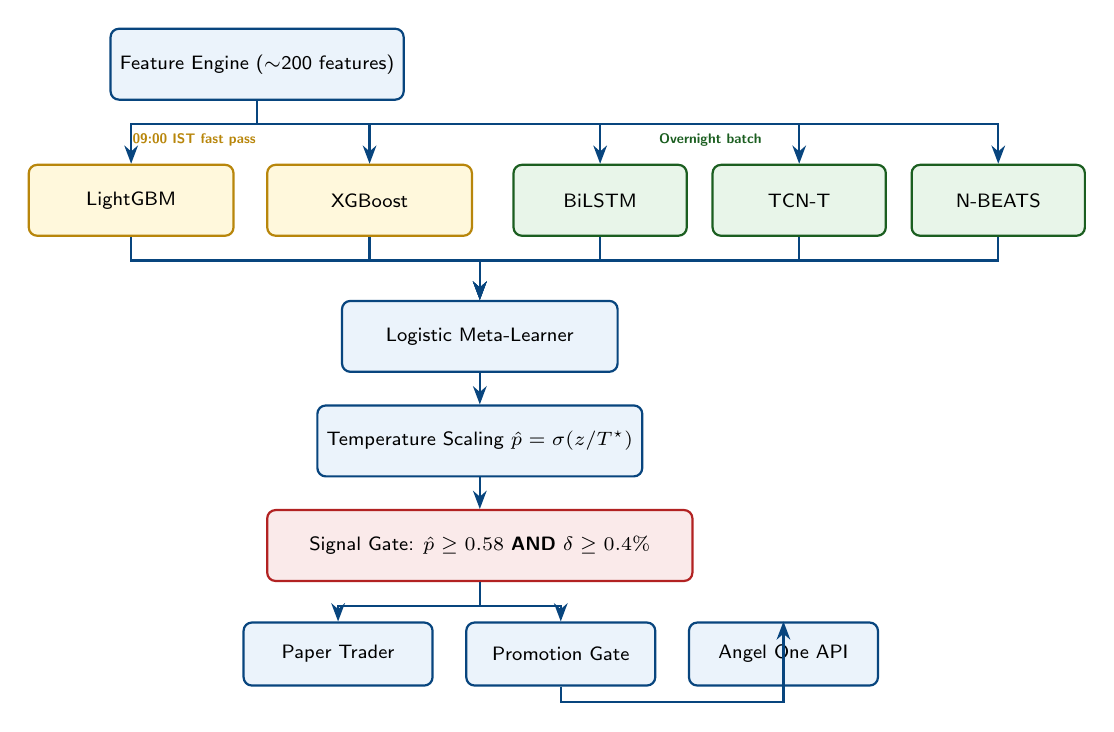
\begin{tikzpicture}[
        node distance=5mm and 7mm,
        every node/.style={font=\scriptsize\sffamily, rounded corners=3pt, align=center},
        stage/.style={draw=primary, fill=blockbg, thick, minimum width=35mm, minimum height=9mm},
        fast/.style={draw=pipelineamber, fill=lightgold, thick, minimum width=26mm, minimum height=9mm},
        dl/.style={draw=pipelinegreen, fill=lightgreen, thick, minimum width=22mm, minimum height=9mm},
        gate/.style={draw=tertiary, fill=lightred, thick, minimum width=54mm, minimum height=9mm},
        live/.style={draw=primary, fill=blockbg, thick, minimum width=24mm, minimum height=8mm},
        arr/.style={-Stealth, thick, draw=primary}
      ]
        \node[stage] (feat) {Feature Engine ($\sim$200 features)};
        \node[fast, below=8mm of feat, xshift=-16mm] (lgbm) {LightGBM};
        \node[fast, right=4mm of lgbm] (xgb)  {XGBoost};
        \node[dl,   right=5mm of xgb]  (bi)   {BiLSTM};
        \node[dl,   right=3mm of bi]   (tc)   {TCN-T};
        \node[dl,   right=3mm of tc]   (nb)   {N-BEATS};
        \node[font=\tiny\bfseries\sffamily, above=1mm of lgbm, xshift=8mm, text=pipelineamber] {09:00 IST fast pass};
        \node[font=\tiny\bfseries\sffamily, above=1mm of bi,   xshift=14mm, text=pipelinegreen] {Overnight batch};
        \node[stage, below=8mm of xgb, xshift=14mm] (meta) {Logistic Meta-Learner};
        \node[stage, below=4mm of meta] (temp) {Temperature Scaling $\hat{p}=\sigma(z/T^\star)$};
        \node[gate,  below=4mm of temp] (gate) {Signal Gate: $\hat{p}\geq 0.58$ \textbf{AND} $\delta\geq 0.4\%$};
        \node[live,  below=5mm of gate, xshift=-18mm] (paper) {Paper Trader};
        \node[live,  right=4mm of paper] (promo) {Promotion Gate};
        \node[live,  right=4mm of promo] (angel) {Angel One API};
        \draw[arr] (feat.south) -- ++(0,-3mm) -| (lgbm.north);
        \draw[arr] (feat.south) -- ++(0,-3mm) -| (xgb.north);
        \draw[arr] (feat.south) -- ++(0,-3mm) -| (bi.north);
        \draw[arr] (feat.south) -- ++(0,-3mm) -| (tc.north);
        \draw[arr] (feat.south) -- ++(0,-3mm) -| (nb.north);
        \draw[arr] (lgbm.south) -- ++(0,-3mm) -| (meta.north);
        \draw[arr] (xgb.south)  -- ++(0,-3mm) -| (meta.north);
        \draw[arr] (bi.south)   -- ++(0,-3mm) -| (meta.north);
        \draw[arr] (tc.south)   -- ++(0,-3mm) -| (meta.north);
        \draw[arr] (nb.south)   -- ++(0,-3mm) -| (meta.north);
        \draw[arr] (meta) -- (temp);
        \draw[arr] (temp) -- (gate);
        \draw[arr] (gate.south) -- ++(0,-3mm) -| (paper.north);
        \draw[arr] (gate.south) -- ++(0,-3mm) -| (promo.north);
        \draw[arr] (promo.south) -- ++(0,-2mm) -| (angel.north);
      \end{tikzpicture}}
      \end{center}
  \end{columns}
\end{frame}

% ── SLIDE 18: FULL STACK ────────────────────────────────────────────────────
\begin{frame}{System Architecture: Full-Stack Dashboard}
  \begin{columns}[T]
    \column{0.36\textwidth}
      \gd{\textbf{Technology Stack}}
      \vsep
      \AS\scriptsize
      \begin{tabular}{@{}p{1.5cm}p{2.6cm}@{}}
        \toprule
        \textbf{Layer} & \textbf{Technology} \\
        \midrule
        Frontend  & Next.js 16, Tailwind, Radix UI, Recharts \\
        Backend   & FastAPI, Uvicorn ASGI \\
        Broker    & Angel One SmartAPI \\
        Data      & Parquet + JSON \\
        Scheduler & APScheduler 09:00 IST \\
        \bottomrule
      \end{tabular}
      \vsep
      \gd{\textbf{Dashboard Modules}}
      \vsep
      \begin{itemize}\itemsep2pt
        \item \textbf{Signal Board}: next-day signals
        \item \textbf{Ledger}: PnL, drawdown chart
        \item \textbf{Gate Panel}: 7-KPI pass/fail
        \item \textbf{Backtest Panel}: equity curve
      \end{itemize}
    \column{0.64\textwidth}
      \begin{center}
      \resizebox{\linewidth}{6.4cm}{%
      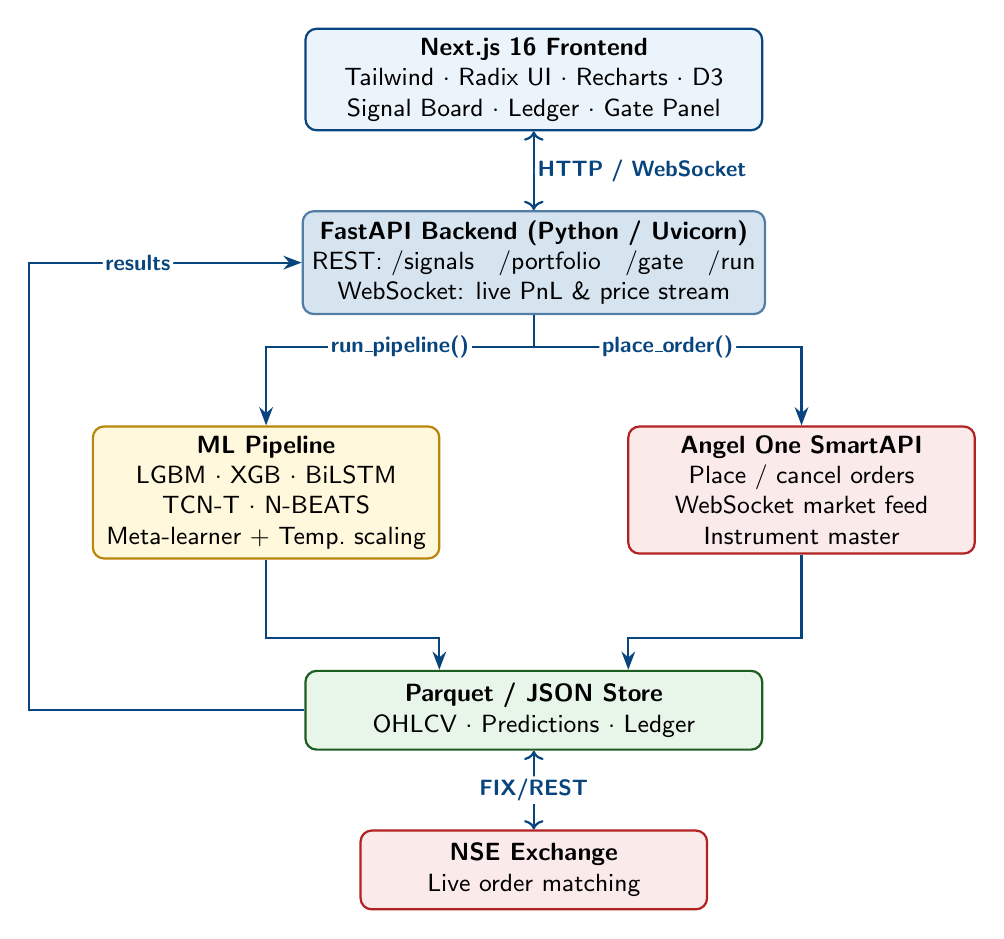
\begin{tikzpicture}[
        every node/.style={font=\small\sffamily, rounded corners=4pt, align=center},
        browser/.style={draw=primary, fill=blockbg, thick, minimum width=58mm, minimum height=10mm},
        api/.style={draw=primary!70, fill=lightprimary, thick, minimum width=58mm, minimum height=10mm},
        pipeline/.style={draw=pipelineamber, fill=lightgold, thick, minimum width=44mm, minimum height=10mm},
        broker/.style={draw=tertiary, fill=lightred, thick, minimum width=44mm, minimum height=10mm},
        store/.style={draw=pipelinegreen, fill=lightgreen, thick, minimum width=58mm, minimum height=10mm},
        arr/.style={-Stealth, thick, draw=primary},
        lbl/.style={font=\footnotesize\bfseries\sffamily, text=primary, fill=white, inner sep=1pt}
      ]
        \node[browser] (ui)   {\textbf{Next.js 16 Frontend}\\Tailwind $\cdot$ Radix UI $\cdot$ Recharts $\cdot$ D3\\Signal Board $\cdot$ Ledger $\cdot$ Gate Panel};
        \node[api,     below=10mm of ui]  (api)  {\textbf{FastAPI Backend (Python / Uvicorn)}\\REST: /signals \; /portfolio \; /gate \; /run\\WebSocket: live PnL \& price stream};
        \node[pipeline,below=14mm of api, xshift=-34mm] (pipe) {\textbf{ML Pipeline}\\LGBM $\cdot$ XGB $\cdot$ BiLSTM\\TCN-T $\cdot$ N-BEATS\\Meta-learner + Temp.\ scaling};
        \node[broker,  below=14mm of api, xshift=34mm]  (brok) {\textbf{Angel One SmartAPI}\\Place / cancel orders\\WebSocket market feed\\Instrument master};
        \node[store,   below=14mm of pipe,xshift=34mm]  (store){\textbf{Parquet / JSON Store}\\OHLCV $\cdot$ Predictions $\cdot$ Ledger};
        \node[broker,  below=10mm of store]             (nse)  {\textbf{NSE Exchange}\\Live order matching};
        \draw[arr,<->] (ui.south) -- node[right,lbl]{HTTP / WebSocket} (api.north);
        \draw[arr] (api.south) -- ++(0,-4mm) -| node[lbl,pos=0.25]{run\_pipeline()} (pipe.north);
        \draw[arr] (api.south) -- ++(0,-4mm) -| node[lbl,pos=0.25]{place\_order()}  (brok.north);
        \draw[arr] (pipe.south) |- ($(store.north)+(-12mm,4mm)$) -- ($(store.north)+(-12mm,0)$);
        \draw[arr] (brok.south) |- ($(store.north)+(12mm,4mm)$) -- ($(store.north)+(12mm,0)$);
        \draw[arr,<->] (nse.north) -- node[lbl]{FIX/REST} (store.south);
        \draw[arr] (store.west) -| ($(pipe.west)+(-8mm,0)$) |- node[lbl,pos=0.7]{results} (api.west);
      \end{tikzpicture}}
      \end{center}
  \end{columns}
\end{frame}

% ── SLIDE 19a: DASHBOARD — OVERVIEW ─────────────────────────────────────────
\begin{frame}{Live Dashboard: Overview}
  \framesubtitle{Next.js 16 + FastAPI; human-in-the-loop monitoring}
  \begin{center}
    \includegraphics[width=\linewidth,height=0.86\textheight,keepaspectratio]{overview.png}
  \end{center}
\end{frame}

% ── SLIDE 19b: DASHBOARD — SIGNALS ──────────────────────────────────────────
\begin{frame}{Live Dashboard: Signal Board}
  \framesubtitle{Next-day calibrated signals with $\hat{p}$, $\delta$, and gate status}
  \begin{center}
    \includegraphics[width=\linewidth,height=0.86\textheight,keepaspectratio]{signals.png}
  \end{center}
\end{frame}

% ── SLIDE 19c: DASHBOARD — PORTFOLIO ────────────────────────────────────────
\begin{frame}{Live Dashboard: Portfolio}
  \framesubtitle{Open positions, exposure, and per-symbol allocation}
  \begin{center}
    \includegraphics[width=\linewidth,height=0.86\textheight,keepaspectratio]{portfolio.png}
  \end{center}
\end{frame}

% ── SLIDE 19d: DASHBOARD — ORDERS ───────────────────────────────────────────
\begin{frame}{Live Dashboard: Orders}
  \framesubtitle{Order book: pending, filled, cancelled with timestamps}
  \begin{center}
    \includegraphics[width=\linewidth,height=0.86\textheight,keepaspectratio]{orders.png}
  \end{center}
\end{frame}

% ── SLIDE 19e: DASHBOARD — SIMULATED PNL ────────────────────────────────────
\begin{frame}{Live Dashboard: Simulated PnL}
  \framesubtitle{Paper-trading equity curve and drawdown}
  \begin{center}
    \includegraphics[width=\linewidth,height=0.86\textheight,keepaspectratio]{simulated_pnl.png}
  \end{center}
\end{frame}

% ── SLIDE 19f: DASHBOARD — 100-STOCK ANALYSIS ───────────────────────────────
\begin{frame}{Live Dashboard: 100-Stock Analysis}
  \framesubtitle{Universe-wide ranking by gate-pass and predicted move}
  \begin{center}
    \includegraphics[width=\linewidth,height=0.86\textheight,keepaspectratio]{100_stock_analysis.png}
  \end{center}
\end{frame}

% ── RESULTS: PER-SYMBOL ─────────────────────────────────────────────────────
\begin{frame}{Results: Per-Symbol Analysis}
  \framesubtitle{Two representative stocks from the 100-symbol panel}
  \begin{columns}[T]
    \column{0.50\textwidth}
      \gd{\textbf{SBIN: Banking (OOS Acc. 0.549)}}
      \vsep
      \begin{itemize}\itemsep3pt
        \item Signals cluster around \textbf{RBI MPC windows} and results seasons
        \item Banking force-include (DXY, Crude, days-to-RBI) adds signal quality
      \end{itemize}
      \begin{center}
        \includegraphics[width=0.80\textwidth]{SBIN_confidence_timeline.png}
      \end{center}
    \column{0.50\textwidth}
      \gd{\textbf{BRITANNIA: FMCG (OOS Acc. 0.563)}}
      \vsep
      \begin{itemize}\itemsep3pt
        \item Top-10 in the 100-symbol panel; LGBM best model (0.594)
        \item Calendar and statistical features dominate importance ranking
      \end{itemize}
      \begin{center}
        \includegraphics[width=0.80\textwidth]{BRITANNIA_oos_accuracy.png}
      \end{center}
  \end{columns}
\end{frame}

% ── CASE STUDIES: PRIOR JOURNAL WORK ────────────────────────────────────────
\begin{frame}{Case Studies: Prior Journal Work}
  \framesubtitle{What top-tier studies did, and what they left undone}
  \AS\scriptsize
  \begin{tabular}{@{}p{2.6cm} p{2.4cm} p{2.0cm} p{3.4cm}@{}}
    \toprule
    \textbf{Study} & \textbf{Method} & \textbf{Validation} & \textbf{Gap addressed here} \\
    \midrule
    Patel et al.\ '15, \textit{Expert Sys.} & ANN, SVM, RF on NSE indicators & Single split & No cost model; no WFV; no calibration \\
    Fischer \& Krauss '18, \textit{EJOR} & LSTM, S\&P~500 daily returns & Walk-forward, no calibration & Per-fold calibration absent; not Indian \\
    Nabipour et al.\ '20, \textit{Entropy} & LSTM, GRU on 4 Tehran sectors & Single split & Accuracy without deployable Sharpe \\
    Long et al.\ '19, \textit{IEEE Access} & DL trading agents, US equities & Random split & No leakage audit; no regime conditioning \\
    L\'opez de Prado '18, \textit{Adv.\ Fin.\ ML} & Methodology (PBO, CSCV, MDA) & --- & Methods used here; not at panel scale in India \\
    Shwartz-Ziv \& Armon '22, \textit{NeurIPS} & Tabular DL vs.\ trees benchmark & --- & Motivates tree weighting in our meta-learner \\
    \bottomrule
  \end{tabular}
  \vsep
  {\footnotesize\textit{Common gaps across this list: (i) no Indian cost stack, (ii) no calibrated probability gate, (iii) no regime-conditional profitability proof, (iv) no live promotion gate. This thesis addresses all four.}}
\end{frame}

% ── CONCLUSION & CONTRIBUTIONS (insights only) ──────────────────────────────
\begin{frame}{Conclusion \& Contributions}
  \framesubtitle{Why this works, what is unique, and what it signifies}
  \begin{columns}[T]
    \column{0.50\textwidth}
      \gd{\textbf{Why the Ensemble Works}}
      \begin{itemize}\itemsep1pt\footnotesize
        \item \textbf{Three orthogonal error sources:} trees, BiLSTM/TCN, N-BEATS; meta-learner weights each per-symbol
        \item \textbf{Calibrated gate} turns 51\% raw into a 57\% \emph{operationally trustworthy} signal --- the gate is the deployable artefact
        \item \textbf{Macro + calendar features} surface conditional structure at regime-change windows (RBI, expiry, results)
        \item Profitability is \textbf{regime-robust}, not a bull-market artefact
      \end{itemize}
    \column{0.50\textwidth}
      \gd{\textbf{Novel Contributions}}
      \begin{enumerate}\itemsep1pt\footnotesize
        \item \textbf{Panel-scale leakage-audited WFV} on 100 NSE stocks (6 folds)
        \item \textbf{Calibrated gating} via temperature scaling --- 58\% has empirical probability meaning
        \item \textbf{Heterogeneous tree + DL committee} with logistic meta-learner on OOF probabilities
        \item \textbf{Full Indian cost-stack backtest} (STT, GST, exchange, SEBI, slippage)
        \item \textbf{7-KPI fail-closed promotion gate} on paper-trading KPIs
      \end{enumerate}
  \end{columns}
  \vspace{0.20cm}
  \begin{exampleblock}{What This Signifies}
    \scriptsize
    Honest accuracy is not the deliverable: a \textbf{calibrated, gated, cost-aware system} is. This thesis reframes NSE stock prediction from a modelling contest into a \textbf{deployment-discipline} problem and provides a reproducible, leakage-audited, regime-conditional template for the Indian market.
  \end{exampleblock}
\end{frame}

% ── SLIDE 23: FUTURE SCOPE ──────────────────────────────────────────────────
\begin{frame}{Future Work}
  \begin{columns}[T]
    \column{0.50\textwidth}
      \gd{\textbf{Immediate Roadmap (next 3 months)}}
      \vsep
      \begin{enumerate}\itemsep3pt
        \item \textbf{Live promotion}: 2 more paper weeks to clear DD ($\leq$10\%) and Brier drift ($\leq$0.05)
        \item \textbf{Per-symbol recalibration}: replace panel-wide 0.58 with per-sector isotonic regression
        \item \textbf{F\&O leg}: route probability into a 1-delta long-call (defined-loss, higher Sharpe)
        \item \textbf{Macro shock test}: replay Feb--Apr 2020; re-tune DD gate after shock evidence
      \end{enumerate}
    \column{0.50\textwidth}
      \gd{\textbf{Longer-Term Directions}}
      \vsep
      \begin{enumerate}\itemsep3pt
        \item \textbf{Residual-target DL}: re-train BiLSTM/TCN-T/N-BEATS on tree-model residual
        \item \textbf{FinBERT-India sentiment}: ProsusAI/finbert fine-tuned on 687 hand-labelled Indian-finance sentences (neg / neu / pos), val acc \gr{\textbf{84.06\%}}, F1 \gr{\textbf{84.10\%}}. Walk-forward integration is the next experiment.
        \item \textbf{RL allocation}: bandit / policy-gradient over gate output; calibrated probability as policy state
        \item \textbf{Alternate universes}: BSE MidCap 150 and SGX Nifty futures; test portability
      \end{enumerate}
  \end{columns}
\end{frame}

% ── SLIDE 24: REFERENCES ────────────────────────────────────────────────────
\begin{frame}{References}
  \vspace{-0.4cm}
  \begin{columns}[T]
    \column{0.50\textwidth}
      \scriptsize
      \begin{itemize}\itemsep1pt
        \item Fama, E.F. (1970). Efficient Capital Markets. \textit{JoF, 25}(2).
        \item Chen, T. \& Guestrin, C. (2016). XGBoost. \textit{KDD} 785--794.
        \item Ke, G. et al. (2017). LightGBM. \textit{NeurIPS} 3149--3157.
        \item Hochreiter, S. \& Schmidhuber, J. (1997). LSTM. \textit{Neural Computation}.
        \item Bai, S. et al. (2018). TCN. \textit{arXiv:1803.01271}.
        \item Oreshkin, B. et al. (2020). N-BEATS. \textit{ICLR}.
        \item Guo, C. et al. (2017). Calibration of Neural Networks. \textit{ICML}.
        \item Wolpert, D.H. (1992). Stacked Generalisation. \textit{Neural Networks, 5}(2).
      \end{itemize}
    \column{0.50\textwidth}
      \scriptsize
      \begin{itemize}\itemsep1pt
        \item Dietterich, T.G. (2000). Ensemble Methods. \textit{MCS 2000}.
        \item L\'opez de Prado, M. (2018). \textit{Advances in Financial ML}. Wiley.
        \item Fischer, T. \& Krauss, C. (2018). Deep learning prediction. \textit{EJOR, 270}(2).
        \item Patel, J. et al. (2015). Predicting Stock Returns. \textit{Expert Systems, 32}(4).
        \item Long, W. et al. (2019). Deep learning stock trading. \textit{IEEE Access, 7}.
        \item Nabipour, M. et al. (2020). DL for stock prediction. \textit{Entropy, 22}(8).
        \item Shah, D. et al. (2019). Stock Market Analysis Review. \textit{IEEE Access, 7}.
        \item Shwartz-Ziv, R. \& Armon, A. (2022). Tabular vs DL. \textit{NeurIPS}.
      \end{itemize}
  \end{columns}
\end{frame}

% ── SLIDE 25: THANK YOU ─────────────────────────────────────────────────────
{
\setbeamertemplate{footline}{}
\begin{frame}[plain]
  \begin{center}
    \vspace{1.0cm}
    {\color{primary}\Large\textbf{Thank You}}\\[0.3cm]
    {\color{secondary}\rule{0.5\textwidth}{0.8pt}}\\[0.4cm]
    {\normalsize\color{primary}\textbf{Vishwam K. Shah}}\\[0.1cm]
    {\small\color{primary!70}Roll No: 24MAI022 $\cdot$ M.Tech AI $\cdot$ PDEU}\\[0.15cm]
    {\small\color{primary!70}Guided by: \textbf{Dr.\ Jigarkumar Shah}, ICT Department}\\[0.5cm]
    {\color{secondary}\rule{0.5\textwidth}{0.4pt}}\\[0.35cm]
    {\normalsize\color{primary!80} Questions \& Discussion Welcome}
  \end{center}
\end{frame}
}

\end{document}
